\chapter{Arquitectura}
\label{chap:arquitectura}

\section{Introducción}
\gotrev{Última revisión 25/06/12}

Este capítulo explicará de forma detallada la estructura del sistema desarrollado usando el estandar UML. Este sistema ha sido implementado usando el lenguaje C++ para todos los módulos, apoyándose de librerías y tecnología detalladas en el Apéndice~\ref{chap:techs}.\\

Se comenzará explicando dos pilares básicos del proyecto: la representación de una imagen analizada y la de una pieza musical, para después describir cada uno de los módulos del proyecto.\\

\subsection{Formato de representación de las figuras}

\todo{Añadir el diagrama y hacer referencia a el cuando una explicación textual no sea suficiente}
Las imágenes vienen representadas por un documento XML  estructurado de la siguiente manera:

\begin{itemize}
\item \textbf{Shapes}: Representa la imagen completa, contiene un listado de las figuras resultantes del análisis.
\item \textbf{Figure}: Contiene la información relativa a una figura.
\item \textbf{Id}: Identificador único de la figura.
\item \textbf{Color}: Identificador para delimitar la información sobre el color.
\item \textbf {RGB}: Identificador para delimitar la información sobre los valores RGB del color.
\item \textbf{R}: Valor referente a la escala de rojo en la escala RGB.
\item \textbf{G}: Valor referente a la cantidad de verde en la escala RGB.
\item \textbf{B}: Valor referente a la cantidad de azul presente en escala RGB.
\item \textbf{VertexList}: Lista de vértices que componen el polígono.
\item \textbf{Vertex [type=``normal'']}: Identificador para delimitar un vértice que pertenece a uno de los extremos de una recta o curva del polígono.
\item \textbf{Position}: Identificador para delimitar la posición de un vértice en la imagen.
\item \textbf{X}: Componente x de la posición del vértice.
\item \textbf{Y}: Componente y de la posición del vértice.
\item \textbf{Vertex [type=``center'']}: Identificador para delimitar un vértice que señala el centro de circunferencia que forma la curva que conecta el vértice anterior a este con el siguiente.
\item \textbf{Area}: Valor numérico del área de una figura.
\item \textbf{Canvas}: Identificador que delimita las figuras situadas dentro de la figura que contiene este elemento. 
\end{itemize}

\todo{Esto es un primer boceto del sistema de clases de figuras que trabaja sobre el XML, técnicamente correcto pero le falta un repaso}

Para poder tratar toda esta información el proyecto dispone de un sistema de clases que permite cargar o guardar y manejar los datos del XML, el siguiente diagrama muestra como está estructurado:
\\\todo{Imagen con el diagrama de Figuras (con o sin phicfigures y mufigures?)}
\newline
\\La clase ``Figura'' esta compuesta por una lista de elementos ``Vertice'', formados por unas coordenadas 'x' e 'y', que determinan su forma, su área y el color expresado en RGB \todo{referencia?}, esto determinaría el polígono al que se refiere. Debido a la procedencia de las figuras y la interpretación que se ha realizado de ellas se dispone también de: un puntero a su figura padre, de estar incluida en otra figura, una lista ordenada arbitrariamente de figuras hijas, en el caso de ser ``padre'' y punteros a las figuras adyacentes a ella según la prioridad que se haya querido tener en cuenta. Además de los elementos mencionados ``Figura'' dispone de la siguiente funcionalidad:
\begin{itemize}
\item \textbf{getSimpleCenter}: Permite adquirir una aproximación del centro del polígono al que representa la figura.
\item \textbf{getBaryCenter}: Permite adquirir el baricentro del polígono al que representa la figura.
\item \textbf{polarize}: Devuelve la figura como una lista de vértices en coordenadas expresadas como un ángulo y longitudes relativas. 
\item \textbf{radialDivision}: Devuelve una división radial de la figura.
\item \textbf{getSaturation}: Calcula el valor de la saturación de la figura.
\item \textbf{isPointInside}: Devuelve si un punto está o no dentro de la figura.
\item \textbf{isFigureInside}: Determina si una figura está o no envuelta por esta.
\end{itemize}
Además también permite el acceso a sus elementos y el manejo de su lista de hijos a través de las funciones pertinentes.
\newline
\todo{mencionar o no las funciones de setParentSon structure, no me queda claro que hacen o si son relevantes para esta parte...}
\\``Figuras'' se caracteriza por tener dos listas de elementos ``Figura'', una con todas las figuras que se le hayan añadido y otra que solo contiene las figuras que están situadas sobre el fondo de la imagen, es decir, que no están envueltas por ninguna otra figura. Además de estos elementos dispone también de la siguiente funcionalidad:
\begin{itemize}
\item \textbf{guardar}: Esta función se encarga de escribir toda la información que contiene en un fichero XML, tras escribir toda la cabecera del fichero se irá recorriendo la lista de figuras padre escribiéndolas como elementos de ``shapes'', cada vez que se escriba una figura se recorrerá su lista de hijas y se irán guardando como elementos de la figura padre en su elemento XML mencionado anteriormente: ``canvas''. \todo{(referencia?)}, de esta manera mantiene la relación padre-hijos en el XML.
\item \textbf{cargar}: Esta función se encargará de leer el fichero XML interpretando su estructura para guardar correctamente la información en figuras, haciendo la distinción de aquellas directamente situadas en ``shapes'' para la segunda lista de figuras y construyendo todos los elementos ``Figura'' con todos sus atributos inicializados a sus valores correspondientes.
\item \textbf{calcularCentro}: Calcula el centro relativo de todas las figuras de la imagen.
\item \textbf{deleteReps}: Borra las figuras repetidas que pueden aparecer como resultado de algunos de los análisis utilizados \todo{referencia}
\item \textbf{redoColorFig}: Vuelve a calcular valores relativos al color de todas las figuras juntas y su variación respecto a las demás. \todo{repasar, no se si es correcto} 
\end{itemize}
Además de lo mencionado anteriormente permite también tratar con sus listas y trabajar con sus elementos.

\subsection{Formato de representación de música}

\todo{Repasar formalizar}

La estructura para representar la música propuesta en el proyecto está determinada por un árbol que trabaja desde el elemento más general, la canción que se va a componer, al más específico, cada una de las notas que componen dicha canción, como muestra la Figura~\ref{fig:structmusic}.\\
	
	\begin{figure}[htbp]
	\centering
	\hspace*{-0.1in}
	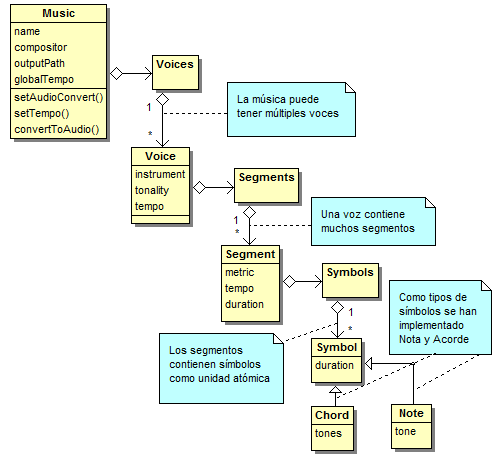
\includegraphics[scale=0.47]{graphics/musica-estructura.png}
	\caption{Estructura de una pieza musical}
	\label{fig:structmusic}
	\end{figure}


\textbf{Música}: Al nivel de la Música, trabajamos con la información relativa a toda la canción que se va a componer, por un lado está información relativa al nombre de la composición y del compositor que la ha hecho, también dispone de una serie de voces a partir de las cuales estará formada la canción y su tempo. Por último a un nivel más cercano, la implementación permitirá elegir con que herramienta querremos crear el archivo de audio de salida.
\newline

\textbf{Voz}: Por debajo de la Música se trabaja con las Voces. Su estructura permite determinar el instrumento, la tonalidad y el tempo de cada una de las voces que componen una pieza, cada una de estas voces esta compuesta de varios segmentos musicales, los cuales al ser reproducidos en el orden establecido por el compositor forman la Voz en cuestión.
\newline

\textbf{Segmento}: Estos elementos tienen la posibilidad de establecer su propia métrica, su tempo y su duración. Los segmentos a su vez están formados por una sucesión de símbolos.
\newline

\textbf{Símbolo}: Son la unidad a partir de la cual se crean todos los elementos básicos de la música, símbolo nos permite establecer una duración para estos elementos. Actualmente el proyecto crea dos tipos de elementos a partir de símbolo:
\begin{itemize}
\item \textbf{Notas}: Estos símbolos tienen asociada una duración, determinada por el componente anterior, y un tono establecido por un número que posteriormente será interpretado con la herramienta que generará el archivo de audio.
\item \textbf{Acordes}: Los acordes están formados de la misma manera que las notas pero en lugar de tener asociado un único tono pueden tener de dos a tres tonos diferentes, en la práctica esto resultará en todos los tonos sonando a la vez durante el mismo tiempo una vez generada la canción.
\end{itemize}
 

\section{Módulo de composición}
\label{sec:modcomp}

\torev{Última revisión realizada el 20-06-2012}

El módulo de composición es el encargado de crear un archivo de audio a partir de un archivo XML con información de figuras. Previo a crear el archivo de audio, será necesario componer la música en base a la configuración del usuario y a los datos de las figuras. La composición se verá plasmada en un fichero ABC siguiendo la notación musical ABC \color{blue}(Apéndice~\ref{sec:NotacionABC})\color{black}. De esta manera nos facilita la conversión en archivos de audio y además la posibilidad de mostrar la partitura de la pieza musical creada.

Para la conversión y manipulación de los archivos de audio se usará los sistemas externos abcMIDI (Apéndice~\ref{sec:abcMIDI}) y Timidity (Apéndice~\ref{sec:Timidity}). abcMIDI se usarán para convertir el archivo generado ABC en formato MIDI y a partir del MIDI se generará el formato WAV de sonido con Timidity. El proyecto de abcMIDI está formado por varios programas de los cuales sólo se utilizará abc2midi.

\subsection{Vista de Implementación}
La implementación realizada sigue el esquema de la Figura~\ref{fig:diagramaclasesMu}.\\

		\begin{figure}[!htbp]
		\centering
		\hspace*{0.0in}
		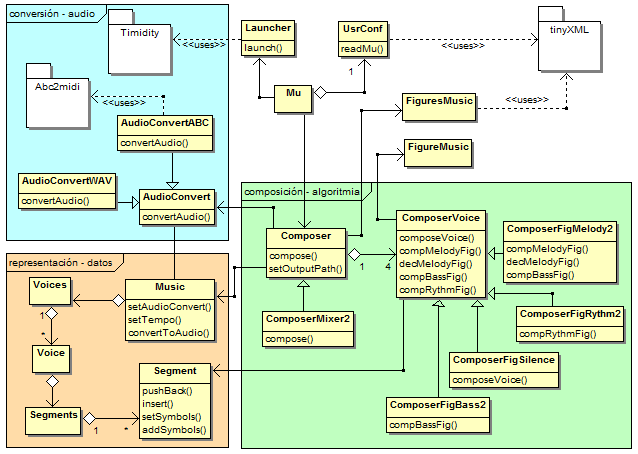
\includegraphics[scale=0.56]{graphics/diagramaclasesMU.png}
		\caption{Diagrama de clases del módulo de Composición}
		\label{fig:diagramaclasesMu}
		\end{figure}

Las clases más importante que podemos observar son:\\

\begin{itemize}

	\item \textbf{Mu:} se trata de la clase que controla la ejecución de este módulo. Se ocupa de crear y coordinar las clases principales de la composición. Además, al final se encarga de llamar al programa Timidity para que realice la conversión de Midi a Wav.
	
	\item \textbf{UsrConf:} como se explica en posteriores secciones, es una clase común que se ocupa de la lectura de los archivos de configuración que el usuario a especificado mediante la interfaz gráfica.
	
	\item \textbf{FiguresMusic:} es necesario crear una clase a partir de Figures que nos brinde una funcionalidad extra necesaria para el módulo de composición. Se explica más adelante los motivos de esta necesidad.
	
	\item \textbf{FigureMusic:} se trata de una extensión de la clase Figure, a la que toma como padre. Se explica más adelante los motivos de su creación.

	\item \textbf{Launcher:} ofrece la funcionalidad para ejecutar una aplicación externa. Se detalla más adelante, en la Sección~\ref{sec:arqMuphic}.

	\item \textbf{TinyXML:} Se trata de un paquete externo de código libre que permite generar y manipular archivos XML.

\end{itemize}

El resto de clases podemos separarlas en tres apartados diferentes según su objetivo principal:\\

Compositores - Algoritmia (color verde Figura~\ref{fig:diagramaclasesMu}):

\begin{itemize}
	
	\item \textbf{Composer:} encargado de procesar las figuras de entrada y crear la estructura de los datos de música. Su principal cometido es componer la música sirviendose de los métodos de composición que albergan los compositores de voces. Otra responsabilidad importante es crear el tipo de conversor adecuado para transformar nuestra notación musical en archivos de audio.

	\item \textbf{ComposerVoice:} la tarea principal de un compositor de voz es crear un segmento de música a partir de una figura de entrada. Existe la posibilidad de componer música para las cuatro diferentes voces identificadas (ver Sección~\ref{sec:algComposicion}). De esta clase extienden los diferentes algoritmos de composición implementados.

	\item \textbf{ComposerFigMelody2:} un ejemplo de clase que extiende de ComposerVoice que implementa la funcionalidad de crear música para las voces primera, segunda y tercera con los métodos compMelodyFig( ), decMelodyFig( ) y compBassFig( ).

	\item \textbf{ComposerFigBass2, ComposerFigRythm2:} se explican con mayor minuciosidad los algoritmos implementados en la Sección~\ref{sec:algComposicion}).

	\item \textbf{ComposerFigSilence:} clase encargada de crear una voz que esté en silencio. Esto ocurre cuando el usuario desactiva alguna de las voces de composición.

	\item \textbf{ComposerMixer2:} clase que hereda de Composer. Es una de las implementaciones realizadas que cumple con los cometidos de los que está encargado la clase padre.

\end{itemize}

Representación - Datos (color salmón Figura~\ref{fig:diagramaclasesMu}):

\begin{itemize}
	
	\item \textbf{Music:} encargado de almacenar la pieza musical que se está componiendo. Además debe comunicarse con AudioConvert para generar el archivo de audio. Esta clase se detalla con mayor detalle en la Sección~\ref{sec:repMusic}.

	\item \textbf{Voices, Voice, Segments:} Todas estas clases se detallan en la Sección~\ref{sec:repMusic}.

	\item \textbf{Segment:} es la unidad sobre la que trabajan los compositores de voces. Se usa como contenedor de las notas creadas por los diferentes algoritmos. Más información en la Sección~\ref{sec:repMusic}.

\end{itemize}

Conversión - Audio (color azul Figura~\ref{fig:diagramaclasesMu}):

\begin{itemize}
	
	\item \textbf{AudioConvert:} la principal función es convertir los datos que se manejan en los compositores dentro del sistema en un archivo de audio que permita reproducirse.

	\item \textbf{AudioConvertABC:} esta clase implementa una posible solución a la conversión entre nuestra notación musical y una salida estandar de audio. En este caso primero se transforma nuestra notación en un archivo con notación ABC y seguidamente se usa la aplicación externa Abc2midi para convertir el archivo ABC en un archivo de sonido Midi

	\item \textbf{AudioConvertWAV:} de forma experimental se desarrolló un sintetizador de sonido que, a partir de nuestra notación, generaba directamente un archivo wav sin compresión. Actualmente no se usa, ya que se obtienen con Abc2midi y Timidity archivos de sonido con mejor calidad y riqueza.

	\item \textbf{Abc2midi:} aplicación externa encargada de convertir un archivo de entrada con formato ABC en un archivo de sonido midi.

	\item \textbf{Timidity:} aplicación externa capaz de repoducir y convertir diferentes formatos de audio. En nuestro sistema se utiliza para convertir el archivo de sonido midi en wav.

\end{itemize}
	
El fujo de ejecución de una composición completa viene representado la Figura~\ref{fig:diagramaflujoMU1} y la Figura~\ref{fig:diagramaflujoMU2} con diagramas de secuencia o flujo. El primer diagrama reproduce la ejecución a alto nivel mientras que el segundo diagrama detalla la parte de ejecución encargada de la composición y conversión a archivo de sonido.

		\begin{figure}[!htbp]
		\centering
		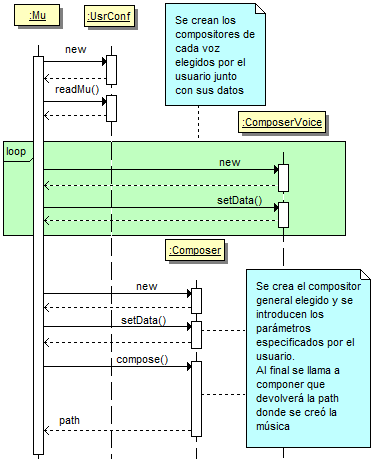
\includegraphics[scale=0.6]{graphics/diagramaflujoMU1.png}
		\caption{Flujo de ejecución alto nivel de abstracción del módulo de composición}
		\label{fig:diagramaflujoMU1}
		\end{figure}

		\begin{figure}[!htbp]
		\centering
		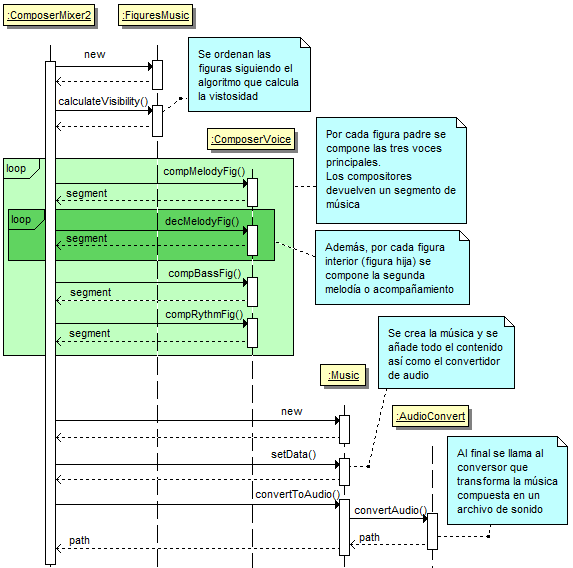
\includegraphics[scale=0.6]{graphics/diagramaflujoMU2.png}
		\caption{Dentro del módulo de composición, flujo de ejecución de los compositores}
		\label{fig:diagramaflujoMU2}
		\end{figure}



%--------------------------------------------------------------------------------------------------------------
\subsection{Figuras Musicales}

El módulo de composición trata las figuras según sus necesidades. Por ello, lo que necesita saber de cada figura además de todos los datos que se encuentran dentro de Figures es la relevancia o vistosidad de cada una, para ello hereda de las clases Figures y Figure mencionadas anteriormente en la Sección~\ref{subsec:usosFigure}, con las clases nuevas llamadas FiguresMusic y FigureMusic (Figura~\ref{fig:diagramaClasesFigureMusic}).

		\begin{figure}[!htbp]
		\centering
		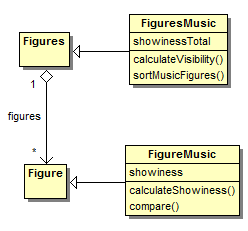
\includegraphics[scale=0.6]{graphics/diagramaClasesFigureMusic.png}
		\caption{Diagrama de las clases Figures y FiguresMusic}
		\label{fig:diagramaClasesFigureMusic}
		\end{figure}

A la clase FigureMusic se le añade la siguiente funcionalidad:

\begin{itemize}

	\item{calcularVistosidad}: Se calcula la relevancia de una figura dentro de una imagen con los siguientes valores: cantidad de rojo de la figura, cantidad de verde de la figura, cantidad de azul de la figura, área de la figura y distancia al centro de la imagen. Cada característica tiene su propio peso. La fórmula que relaciona todas estas características se ve con detalle en la Sección~\ref{sec:algComposicion}. Es necesario este valor para poder clasificar las figuras y así los compositores puedan usar las figuras de forma organizada.

	\item{compare}: Compara dos figuras según el valor de la vistosidad. Si dos figuras tienen misma vistosidad entonces tienen misma relevancia dentro de la imagen. Se emplea para poder ordenar las figuras.

\end{itemize}

A FiguresMusic se le añaden los elementos necesarios para poder considerar y utilizar la nueva funcionalidad añadida a FigureMusic:

\begin{itemize}

	\item{calcuteVisibility}: Primero calcula la vistosidad de cada figura si es que no se ha calculado ya, tomando los valores. Después se normalizan esos valores teniendo en cuenta el total de todas las figuras y la media. Función que usa sortMusicFigures para poder después ordenar las figuras.

	\item{sortMusicFigures}: Dada una lista de figuras, devuelve la lista ordenada según la vistosidad de las figuras. Esta funcionalidad se utiliza por parte de los compositores, para ordenar las figuras por su criterio de relevancia dentro de la imagen.

\end{itemize}
\section{Módulo de análisis}

\todo{referenciar figuras,	analizer, uso de opencv como paquete}


El módulo de análisis, como ya se ha comentado, es el encargado de, dada una imagen dada y una configuración de entrada, producir un archivo XML con la lista de polígonos que componen la imagen. Esta lista debe componer una nueva imagen lo más fiel posible a la imagen de entrada, teniendo en cuenta los ajustes especificados en el archivo de configuración.\\

Este módulo hace un gran uso de la librería externa OpenCV, de la cual se ayuda tanto para tratar imágenes como para componer formas y polígonos.

\subsection{Vista de implementación}

La estructura general del módulo se ve en la Figura~\ref{fig:diagramaclasesPHIC}.\\

		\begin{figure}[htbp]
		\centering
		
\includegraphics[scale=0.47]{graphics/todo.png}
		\caption{Vista de las clases del módulo de anális}
		\label{fig:diagramaclasesPHIC}
		\end{figure}
		
	\todo{este diagrama contiene el nombre de ciertas funcionas (las que aparecen en el diagrame de flujo)}
		
En ella, se pueden observar las siguientes clases:\\

\begin{itemize}

	\item \textbf{Phic:} Se trata de la clase que controla la completa ejecución de este módulo. Se ocupa de coordinar el resto de clases para que realicen las operaciones requeridas para completar el análisis.
	
	\item \textbf{Analizer:} realiza todas las operaciones de análisis y se comunica con la librería OpenCV.
	
	\item \textbf{UsrConf:} como se explica en posteriores secciones, es una clase común que se ocupa de la lectura de los archivos de configuración.
	
	\item \textbf{TinyXML:} Se trata de un paquete externo de código libre que permite generar y manipular archivos XML.
	
\end{itemize}	
			
El flujo de ejecución de un análisis cualquiera realizado con este módulo se ve en la Figura~\ref{fig:diagramaflujoPHIC}.\\

		\begin{figure}[htbp]
		\centering
		
\includegraphics[scale=0.47]{graphics/todo.png}
		\caption{Flujo de ejecución del módulo de anális}
		\label{fig:diagramaflujoPHIC}
		\end{figure}
		
\todo{resumen pequeño que se hace mucho mas rapido con el diagrama ya hecho}
		
\subsection{Vista de despliegue}
\todo{puede que sobre porque es obvio y UBERrepetitivo, pero es para que se vea que opencv está como dll ahí}
		
Por último, la vista final del módulo como paquetes se ve en la Figura~\ref{fig:diagramapaquetesPHIC}.\\

		\begin{figure}[htbp]
		\centering
		
\includegraphics[scale=0.47]{graphics/todo.png}
		\caption{Diagrama de paquetes del módulo de anális}
		\label{fig:diagramapaquetesPHIC}
		\end{figure}
		
El sistema se basa en la librería externa OpenCV para relizar sus funciones.
\subsection{Módulo de conexión}

\todo{hablar de muphic}

\subsection{Interfaz Gráfica}

\todo{rehacer reusando parte de esto:

El desarrollo de la interfaz gráfica se decidió realizar a través de un framework que facilitase la construcción de la misma. Qt, la herramienta que se utilizó se eligió debido a dos criterios, era multiplataforma, al igual que la aplicación, servía para trabajar con móviles, siguiendo así uno de los enfoques iniciales del proyecto que más adelante fue descartado. Además Qt trabaja con C++ como lenguaje de programación, el mismo que el núcleo de la aplicación y ofrece facilidades a la hora de integrar audio, a través de la librería Phonon, o componentes personalizados en una interfaz.\\
\todo{Este párrafo no se si abriría mejor la parte de arquitectura}
\newline
La interfaz esta compuesta de tres pestañas cada una encargada de una parte de la funcionalidad:

\underline{Composition Config:}
\\En esta pestaña se pueden encontrar todas las opciones disponibles para el compositor musical, estás serán transmitidas a los módulos de la aplicación cuando se pulse el botón de "Compose" en la "Main Window" a través del documento XML mencionado anteriormente.
\\Como se puede ver en la imagen adjunta, hay opciones para cuatro voces, que son aquellas con las que trabajan los compositores de la aplicación siendo, normalmente, la "Voice 1" la melodía principal, la "Voice 2" un acompañamiento, la "Voice 3" el bajo y la "Voice 4" la percusión. Las opciones disponibles son las siguientes:
\\\todo{Adjuntar imagen}
\newline
\\textit{Color System:} Hace referencia referencia a la teoría sinestésica que se utilizará como base para la relación de color-notas durante la composición musical.
\\textit{Composer:} En las cuatro voces se refiere a que compositor se utilizará para esa voz, al presionarlo se desplegarán los distintos compositores que están disponibles para que el usuario elija el que mejor le convenga.
\\textit{Instrument:} En las cuatro voces se refiere a que instrumento se utilizará para esa voz en concreto, al presionarlo se desplegarán los instrumentos disponibles.
\\textit {Composer Mixer:} Hace referencia a que como se combinarán las cuatro voces anteriores.
\\textit{Tempo:} 
\\\todo{A rellenar con gente que sepa describirlo mejor que yo. \\También hay que repasar lo anterior}
\newline
\\{\bf Libreria Phonon}
\\Esta es una librería proporcionada por Qt para la reproducción de audio, al ser un módulo externo requiere una serie de librerías añadidas que están incluidas en el paquete de instalación de windows, sin embargo tendrán que ser instaladas en linux utilizando alguno de los gestores de software disponibles realizando una búsqueda con la palabra clave: Phonon.
\\Las librerías requeridas son las siguientes: (LISTA DE LIBRERÍAS)
\\En el caso de que no funcione el sistema de reproducción, se pueden encontrar los archivos de audio en la ruta especificada en "Midi Output"
\newline
\\\todo{Claramente esta parte va en arquitectura, sin embargo no se que más comentar de la arquitectura de la GUI puesto que casi todo esta hecho con QT, como no digamos el widget de carlos...}
\\La interacción con phonon se realiza utilizando la funcionalidad proporcionada por el framework. Se asocia el fichero multimedia a un tipo proporcionado por Phonon que a su vez lo conecta con el sistema de audio predeterminado para cada sistema operativo.
\\El uso de Phonon es conveniente porque a pesar de sus complicaciones ofrece una manera sencilla de incluir un reproductor en la interfaz, que a su vez, es multiplataforma sin obligar al usuario a buscar el archivo de audio o forzar una llamada a un tercer programa que reproducir la música que generada.

\subsubsection{Uso de la librería Qt}

\todo{Hacer, usar parte de 3.3.6}

\subsubsection{Vista general}

\todo{Hacer, usar parte de 3.3.6}

\subsubsection{Widget Gráfico}

\todo{Hacer}

\subsubsection{Uso de la librería Phonon}

\todo{Hacer, usar parte de 3.3.6}

La interfaz para poder reproducir los archivos de audio generados hace uso de una librería externa proporcionada por Qt, se trata de Phonon \cite{phononOverview}. }